\documentclass[12pt]{article}

\usepackage{fullpage}
\usepackage{mdframed}
\usepackage{colonequals}
\usepackage{algpseudocode}
\usepackage{algorithm}
\usepackage{tcolorbox}
\usepackage[all]{xy}
\usepackage{proof}
\usepackage{mathtools}
\usepackage{bbm}
\usepackage{amssymb}
\usepackage{amsthm}
\usepackage{amsmath}
\usepackage{amsxtra}
\newcommand{\bb}{\mathbb}


\newtheorem{theorem}{Theorem}[section]
\newtheorem{corollary}{Corollary}[theorem]
\newtheorem{lemma}{Lemma}

\newcommand{\mathcat}[1]{\textup{\textbf{\textsf{#1}}}} % for defined terms

\newenvironment{problem}[1]
{\begin{tcolorbox}\noindent\textbf{Problem #1}.}
{\vskip 6pt \end{tcolorbox}}

\newenvironment{enumalph}
{\begin{enumerate}\renewcommand{\labelenumi}{\textnormal{(\alph{enumi})}}}
{\end{enumerate}}

\newenvironment{enumroman}
{\begin{enumerate}\renewcommand{\labelenumi}{\textnormal{(\roman{enumi})}}}
{\end{enumerate}}

\newcommand{\defi}[1]{\textsf{#1}} % for defined terms

\theoremstyle{remark}
\newtheorem*{solution}{Solution}

\setlength{\hfuzz}{4pt}

\newcommand{\calC}{\mathcal{C}}
\newcommand{\calF}{\mathcal{F}}
\newcommand{\C}{\mathbb C}
\newcommand{\N}{\mathbb N}
\newcommand{\Q}{\mathbb Q}
\newcommand{\R}{\mathbb R}
\newcommand{\Z}{\mathbb Z}
\newcommand{\F}{\mathbb F}
\newcommand{\br}{\mathbf{r}}
\newcommand{\RP}{\mathbb{RP}}
\newcommand{\CP}{\mathbb{CP}}
\newcommand{\nbit}[1]{\{0, 1\}^{#1}}
\newcommand{\bits}{\{0, 1\}^{n}}
\newcommand{\bbni}{\bigbreak \noindent}
\newcommand{\norm}[1]{\left\vert\left\vert#1\right\vert\right\vert}
\newcommand{\dbar}{\overline{\partial}}
\let\d\relax
\let\calF\relax
\newcommand{\d}{\partial}
\newcommand{\calO}{\mathcal{O}}
\newcommand{\calF}{\mathcal{F}}
\newcommand{\calG}{\mathcal{G}}
\newcommand{\calH}{\mathcal{H}}
\newcommand{\calE}{\mathcal{E}}

\let\1\relax
\newcommand{\1}{\mathbf{1}}
\newcommand{\fr}[2]{\left(\frac{#1}{#2}\right)}

\newcommand{\vecz}{\mathbf{z}}
\newcommand{\vecr}{\mathbf{r}}
\DeclareMathOperator{\Cinf}{C^{\infty}}
\DeclareMathOperator{\Id}{Id}

\DeclareMathOperator{\Alt}{Alt}
\DeclareMathOperator{\ann}{ann}
\DeclareMathOperator{\codim}{codim}
\DeclareMathOperator{\End}{End}
\DeclareMathOperator{\Hom}{Hom}
\DeclareMathOperator{\id}{id}
\DeclareMathOperator{\M}{M}
\DeclareMathOperator{\Mat}{Mat}
\DeclareMathOperator{\Ob}{Ob}
\DeclareMathOperator{\opchar}{char}
\DeclareMathOperator{\opspan}{span}
\DeclareMathOperator{\rk}{rk}
\DeclareMathOperator{\sgn}{sgn}
\DeclareMathOperator{\Sym}{Sym}
\DeclareMathOperator{\tr}{tr}
\DeclareMathOperator{\img}{img}
\DeclareMathOperator{\CandE}{CandE}
\DeclareMathOperator{\CandO}{CandO}
\DeclareMathOperator{\argmax}{argmax}
\DeclareMathOperator{\first}{first}
\DeclareMathOperator{\last}{last}
\DeclareMathOperator{\cost}{cost}
\DeclareMathOperator{\dist}{dist}
\DeclareMathOperator{\path}{path}
\DeclareMathOperator{\parent}{parent}
\DeclareMathOperator{\argmin}{argmin}
\DeclareMathOperator{\excess}{excess}
\let\Pr\relax
\DeclareMathOperator{\Pr}{\mathbf{Pr}}
\DeclareMathOperator{\Exp}{\mathbb{E}}
\DeclareMathOperator{\Var}{\mathbf{Var}}
\let\limsup\relax
\DeclareMathOperator{\limsup}{limsup}
%Paired Delims
\DeclarePairedDelimiter\ceil{\lceil}{\rceil}
\DeclarePairedDelimiter\floor{\lfloor}{ \rfloor}


\newcommand{\dagstar}{*}

\newcommand{\tbigwedge}{{\textstyle{\bigwedge}}}
\setlength{\parindent}{0pt}
\setlength{\parskip}{5pt}


\begin{document}

\title{CS 40: Computational Complexity}

\author{Sair Shaikh}
\maketitle

Collaboration Notice: Talked to Henry Scheible '26 to discuss ideas.


\begin{problab}{1}
    Suppose that $f: X \to Y$ is a homotopy equivalence. Show that the map $\pi_0(f): \pi_0(X) \to \pi_0(Y)$ from Homework 1, Problem 5 is a bijection.
\end{problab}
\begin{solu}

\end{solu}
\newpage

\begin{problab}{2}
    (0.11) Show that a continuous map $f: X \to Y$ is a homotopy equivalence if there exist continuous maps $g, h: Y \to X$ such that $f\circ g \simeq \id_Y$ and $h \circ f \simeq \id_X$. More generally, show that $f$ is a homotopy equivalence if $f \circ g$ and $h \circ f$ are homotopy equivalences.
\end{problab}
\begin{solu}
    
\end{solu}
\newpage

\begin{problab}{3}
    Suppose that $G$ is a group and $G_1, \hdots, G_n$ are subgroups that generate $G$ such that $G_i \cap G_j = \{ 1 \}$ for $i \neq j$. Show that $G$ is the free product $G_1 * \hdots * G_n$ if and only if for every group $H$ and collection of homomorphisms $h_j : G_j \to H$, there exists a unique homomorphism $h: G \to H$ such that $h_j = h \circ i_j$ where $i_j: G_j \to G$ is the inclusion.
\end{problab}
\begin{solu}

\end{solu}
\newpage

\begin{problab}{4}
    Find the fundamental group of each arrangement of three spheres below.
    \begin{enumerate}
    \item A chain. 
    \begin{center} 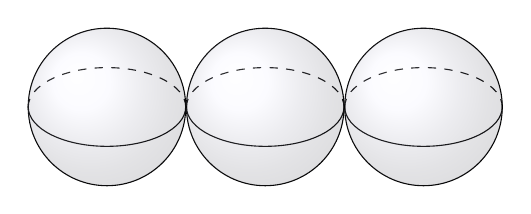
\begin{tikzpicture}
        \draw (-1,0) arc (180:360:1cm and 0.5cm);
        \draw[dashed] (-1,0) arc (180:0:1cm and 0.5cm);
        \draw (0,0) circle (1cm);
        \shade[ball color=blue!10!white,opacity=0.20] (0,0) circle (1cm);
        
        \begin{scope}[xshift = 2.01cm]
            \draw (-1,0) arc (180:360:1cm and 0.5cm);
        \draw[dashed] (-1,0) arc (180:0:1cm and 0.5cm);
        \draw (0,0) circle (1cm);
        \shade[ball color=blue!10!white,opacity=0.20] (0,0) circle (1cm);
        \end{scope}
        
        \begin{scope}[xshift = -2.01cm]
            \draw (-1,0) arc (180:360:1cm and 0.5cm);
        \draw[dashed] (-1,0) arc (180:0:1cm and 0.5cm);
        \draw (0,0) circle (1cm);
        \shade[ball color=blue!10!white,opacity=0.20] (0,0) circle (1cm);
        \end{scope}
      \end{tikzpicture}
      \end{center}
    \item A triangle.
    \begin{center} 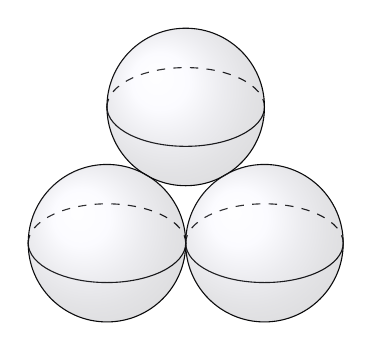
\begin{tikzpicture}
        \draw (-1,0) arc (180:360:1cm and 0.5cm);
        \draw[dashed] (-1,0) arc (180:0:1cm and 0.5cm);
        \draw (0,0) circle (1cm);
        \shade[ball color=blue!10!white,opacity=0.20] (0,0) circle (1cm);
        
        \begin{scope}[xshift = 1 cm, yshift= -1.73 cm]
            \draw (-1,0) arc (180:360:1cm and 0.5cm);
        \draw[dashed] (-1,0) arc (180:0:1cm and 0.5cm);
        \draw (0,0) circle (1cm);
        \shade[ball color=blue!10!white,opacity=0.20] (0,0) circle (1cm);
        \end{scope}
        
        \begin{scope}[xshift = -1cm, yshift=-1.73 cm]
            \draw (-1,0) arc (180:360:1cm and 0.5cm);
        \draw[dashed] (-1,0) arc (180:0:1cm and 0.5cm);
        \draw (0,0) circle (1cm);
        \shade[ball color=blue!10!white,opacity=0.20] (0,0) circle (1cm);
        \end{scope}
      \end{tikzpicture}
      \end{center}
    \end{enumerate}
\end{problab}
\begin{solu}

\end{solu}
\newpage

\begin{problab}{5}
    (1.2.3) Let $X$ be the union of $n$ lines through the origin in $\R^3$. Compute the fundamental group of $\R^3 \setminus X$. 
\end{problab}
\begin{solu}

\end{solu}
\newpage

\end{document}